\documentclass[../ClassicThesis.tex]{subfiles}
\begin{document}

%************************************************
\chapter{Classifiers}\label{ch:classifiers}
\newcommand{\TODO}[1]{\textcolor{red}{\\ \textbf{TODO:} #1 \\}}
%************************************************

\section{Classifiying Idea}
\cite{positionVectorRetrieval}
In the previous chapters we covered the approach of solely finding plates within 3D models. This approach needs the model to be 'boxy'. Therefore sometimes the algorithm fails because of too many round edges or other noise. \\
This is why we tried another approach, called RANSAC \cite{ransac}, which is also being used by CGAL \cite{cgal}. We look for all kinds of primitive shapes in addition to plates. This allows us to split the model into separate objects that can then be independently converted to laser cutable plates. During the conversion we choose a specific method to realise this part with plates which often helps to achieve a more appropriate solution than to directly start finding plates. Due to the tolerance of the algorithm to noise we can even detect surface when there is a lot of texture.
Currently, our software system does not finding the classifiers for a conversion. Instead we wanted to find out how well the algorithm works for our use case. \\
In order to properly include the classifiers we built a theoretical structure to make the most of the findings. \\
A Classifier finds a particular shape like a plane, plate, box, sphere, cylinder, prism, etc. Classifiers can use findings of others for example the box finder depends on the previously found planes. As soon as all classifiers have finished their process all findings are hierarchichally grouped based on the depencies of the classifiers. Each finding is represented as a \emph{graphObject} which can either be of the type volume, like a box or cylinder for example, or a freeform. Freeforms are objects that could not be classified. Nevertheless we check if this object is some kind of connector of volumes. This is valuable information for the conversion step because it means there needs to be something between specified volumes this can be anything that the conversion method might choose. Then a graph is created which keeps all objects and their connections. Finally, the reconstruction starts: Each volume will be converted by its specific converter. The box converted is an example. Connectors will result in plates which are connected to all volumes it belongs to. And from  unclassified objects we create plates based on the shapes found in this part of the mesh. \\
\*\\
% \paragraph{What is it usually used for? - pointclouds... which points do we intend to take for the algorithm?}
Usually, RANSAC is used with pointclouds. This means we need a lot of points and the more noise there is within the points the better for the algorithm. We work with meshes where a model of a box might only have 8 points. This is a problem because the diagonals of the box look just like another plane to the algorithm because the sides and the diagonals are supported by 4 points. 
On the other hand, when this box consisted of thousands of points they would all be somewhere on the sides. Meaning that the diagonal would not be found as a plane because it is maybe only supported by up to 10 points. In contrast, each side is supported by up to hundreds of points. Therefore, the RANSAC approach can not be used with every 3D model. Instead it should be used as an additional option to split the model.
\section{RANSAC - Random Sample Consensus}
The RANSAC-approach firstly chooses a defined number of random points. These points are a subset from the point data and its number is defined by the shape that has been classified. This subset should be choses as small as possible.\\
On the basis each of these minimal sets a candidate shape is generated and tested against all points in the data set. The candidate gets a score which tells how well the randomly chosen points represent the shape. This score can result from counting the points which lie within the candidate.\\
Based on this score the best model is saved or overwritten after several candidate attempts.
\section{Primitives}
In order to classify primitives, a minimum number of points has to be defined to enable a shape reconstruction.
\subsection{Plane Classifier}
The minimal set for a plane consists of three points \{p1, p2, p3\} because three points uniquely identify a plane.\\
Once a plane candidate has been found it is necessary to check its plausibility. The deviations of the plane normal to the according point normals of p1, p2 and p3 should be less than an angle $\alpha$, currently set to 0.1 .\\
\*\\
After the detection of the best model it may be necessary to refit the candidate to all its inliers. We use the Least Squares method \cite{leastSquares}. We are aware that this method can only compute planes where its z-values are dependent on the x- and y-values this is not the case the the plane is perpendicular to the x-y-plane. Therefore we ignore planes to that are affected by this circumstance. Another possibility would be to work with eigenvectors where this would not be an issue.\\
When using the least squares method the problem can be transformed into an equation of the form Ax = b. Where A is a matrix consisting of the sum of all x values of the points, y values, x times y and x squared and y squared. \\

%sums
\begin{bmatrix}
\sum_{i=1}^m x_i^2 & \sum_{i=1}^m x_iy_i & \sum_{i=1}^m x_i\\
\sum_{i=1}^m x_iy_i & \sum_{i=1}^my_i^2 & \sum_{i=1}^m y_i\\
\sum_{i=1}^m x_i & \sum_{i=1}^m y_i & \sum_{i=1}^m 1
\end{bmatrix}
%
%coeffitients
\begin{bmatrix}
A\\
B\\
C
\end{bmatrix}
%
=
%
%solution
\begin{bmatrix}
\sum_{i=1}^m x_iz_i\\
\sum_{i=1}^m y_iz_i\\
\sum_{i=1}^m z_i
\end{bmatrix}


The least squares solution is the following plane equation: \\
$z = Ax + By + C$.

\subsection{Cylinder Classifier}
The minimal set for a cylinder consists of two points \{$p_1, p_2$\}. In Figure~\ref{fig:cylinder} the reconstruction process is sketched. Those randomly picked points are assumed to lie on the shell of the cylinder. If they are not actually lying on the shell then later there will not be enough candidates to support the cylinder which means it will be discarded. The axis can be calculated by calculating the cross product of their normals $n_1$ and $n_2$. Based on the axis a projection plane is formed which is perpendicular to the axis. The two lines $l_1 = p_1 + x*n_1$ and $l_2 = p_2 + x*n_2$ are projected onto this plane and should have an intersection. If they do not intersect the candidate is invalid. Otherwise, the intersection point is marked as the center of the cylinder-candidate. The radius is the mean value of the distance of both points to the center on the axis.
\begin{figure}[!ht]
    \centering
    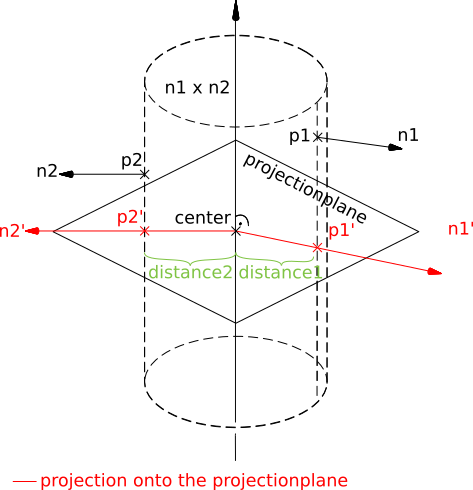
\includegraphics[width=\columnwidth]{Images/cylinder.png}
    \caption{Two points are enough to represent a cylinder. The axis can be reconstructed, as well as the radius.}
    \label{fig:cylinder}
\end{figure}

After a valid candidate has been formed we have to check the plausibility. For this we look for three indicators. Firstly, the randomly chosen points p1 and p2 should not equal, secondly, the calculated radius has to be larger than zero and lastly, the distances of the two points to the center should not exceed an epsilon value $\epsilon$.




\subsection{Prism Classifier}
\label{ch:classifiers-prism}

A Prism is a base element for many other primitives which are characterized by two parallel shapes. Therefore a prism datastructure contains two shapes and the lateral surface as a set of primitives which are usually faces or shapes.

To find the prisms all shapes have to be checked for parallelism. The comparison is based on normals which are sorted into buckets to speed up the process. The attached lateral surface can be identified by flood fill.

\subsubsection{Bucket System}
\label{sec:PrismBucketSystem}

The surface normals $\vec{n}$ are sorted into buckets to reduce the amount of comparisons. Treating slightly different normals as equal considering a given threshold $\phi$ each bucket covers this angle. Therefore to check for similarity only normals within a bucket and the surrounding ones have to be considered: The angle between two normals is always greater $\phi$ if their buckets are not neighbors. The corresponding bucket for a normal is determined by two values $\alpha$ and $\beta$. Their calculation is explained below.

\begin{equation*}
    \vec{n} = (x, y, z)
\end{equation*}


All normals lie on the surface of the unit sphere because of their normalisation. Considering opposite normals as equal like planes with normals $(1,0,0)$ and $(-1,0,0)$ are parallel, all normals are transformed into a hemisphere as shown in Listing~\ref{lst:_normalInHemisphere}: A normal is negated in case its $z$ value is negative.


\begin{listing}[!h]
\centering
\begin{minted}[
linenos
]{coffeescript}
_normalInHemisphere: (normal) ->
    if normal.z < 0
        return normal.clone().negate()
    else
        return normal
\end{minted}
\caption{Normals are transformed into hemisphere}
\label{lst:_normalInHemisphere}
\end{listing}

\begin{figure}
    \includegraphics[width=0.9\columnwidth]{Images/PrismCl-Rings.png}
    \caption{Rings visualised from side}
    \label{fig:rings_FromSide}
\end{figure}

\begin{figure}
    \includegraphics[width=0.9\columnwidth]{Images/PrismCl-RingsFromTop.png}
    \caption{Rings visualised from top}
    \label{fig:rings_FromTop}
\end{figure}

\begin{figure}
    \includegraphics[width=0.4\columnwidth]{Images/PrismCl-RingAngle.png}
    \caption{Angle of a normal which is used for sorting it into a ring}
    \label{fig:ringAngle}
\end{figure}


This hemisphere is separated into rings. Each ring covers the threshold angle $\phi$ in $z$-direction and is visualized in Figure~\ref{fig:rings_FromSide} and Figure~\ref{fig:rings_FromTop}. Each normal is sorted into a ring by its correlating angle $\alpha$ which is used to determine the ring index. It is proporional to its coordinates as demonstrated in Figure~\ref{fig:ringAngle}: the angle between $\vec{n}$ and $(x,y,0)$:

\begin{equation*}
\begin{split}
    \sin{\alpha} & = \frac{z}{ \sqrt{x^{2} + y^{2}} } \\
    => \alpha  & = \arcsin{ \frac{z}{ \sqrt{x^{2} + y^{2}} } }
\end{split}
\end{equation*}


The angle $\alpha$ is represented as a multiple of the threshold angle $\phi$ to get the actual ring index $I_{Ring}$:

\begin{equation*}
    I_{Ring} = \floor*{
                    \arcsin{
                        \frac{z}{ \sqrt{ x^{2} + y^{2} } }
                    }
                    / \phi
                }
\end{equation*}

The maximum angle is 90°. Consequently the maximum ring index $I_{MaxRing}$ is calculated as follows:

\begin{equation*}
    I_{MaxRing} = \floor*{
                    \frac{\pi}{2}
                    / \phi
                  }
\end{equation*}



The angle in the middle of each ring ${\alpha}_{I_{Ring}}$ consequently depends on index and threshold:

\begin{equation}
\label{equ:AlphaIRing}
    {\alpha}_{I_{Ring}} = (I_{Ring} + 0.5) * \phi \qquad \forall{ I_{Ring} \in [0, I_{MaxRing}] }
\end{equation}



Figure~\ref{fig:middleZ} implies the calculation of the corresponding middle $z$ value $z_{I_{Ring}}$: We create a normal $\vec{a}_{I_{Ring}}$ with a fixed $y$ value of 0 that forms the angle ${\alpha}_{I_{Ring}}$ with the unit vector in x direction $\vec{v}_{x}$. Consequently all normals that lie in the middle of a ring ($\alpha = {\alpha}_{I_{Ring}}$) have the $z$ value $z_{I_{Ring}}$.

\begin{figure}
    \includegraphics[width=0.5\columnwidth]{Images/PrismCl-MiddleZ.png}
    \caption{Geometric visualization of the z value in the middle of a ring}
    \label{fig:middleZ}
\end{figure}

\begin{equation}
\label{equ:VecX}
    \vec{v}_{x} = (1, 0, 0)
\end{equation}

\begin{equation}
\begin{split}
    \label{equ:VecA}
    \vec{a}_{I_{Ring}} = (x_{a}, 0, z_{I_{Ring}}) \qquad  & \forall{ I_{Ring} \in [0, I_{MaxRing}] } \\
    & with \vert \vec{a}_{I_{Ring}} \vert = 1
\end{split}
\end{equation}

\begin{equation}
    \label{equ:XA}
    \cos{{\alpha}_{I_{Ring}}} = \frac{ \vec{v}_{x} * \vec{a}_{I_{Ring}} }{ \vert \vec{v}_{x} \vert * \vert \vec{a}_{I_{Ring}} \vert }
    \stackrel{(\ref{equ:VecX}) + (\ref{equ:VecA})}{=} \vec{v}_{x} * \vec{a}_{I_{Ring}}
    \stackrel{(\ref{equ:VecX}) + (\ref{equ:VecA})}{=} x_{a}
\end{equation}

\begin{equation}
\label{equ:ZIRing}
\begin{split}
    1 & = \vert \vec{a}_{I_{Ring}} \vert \stackrel{(\ref{equ:VecA})}{=} \sqrt{ x_{a}^{2} + z_{I_{Ring}}^{2} } \\
    => z_{I_{Ring}} & = \sqrt{1 - x_{a}^{2}}
    \stackrel{(\ref{equ:XA})}{=} \sqrt{1 - cos^{2}{{\alpha}_{I_{Ring}}}}
\end{split}
\end{equation}


Each ring is seperated into buckets which cover the threshold angle $\phi$ as shown in Figure~\ref{fig:PrismCl-buckets}. Therefore the onto the xy-plane projected angle $\gamma$ needs to be calculated which differs from ring to ring. This is shown in Figure~\ref{fig:projection} and leads to the following calculation.

\begin{figure}
    \includegraphics[width=0.7\columnwidth]{Images/PrismCl-buckets.png}
    \caption{Buckets in a ring span the angle~$\phi$}. Its projection is the angle~ $\gamma$.
    \label{fig:PrismCl-buckets}
\end{figure}


\begin{figure}
    \includegraphics[width=1.0\columnwidth]{Images/PrismCl-Projection.png}
    \caption{Projection of the angle $\protect\phi$}
    \label{fig:projection}
\end{figure}


$ \vec{a}_{I_{Ring}}' $ is the projection of $\vec{a}_{I_{Ring}} $:


\begin{equation}
    \label{equ:VecAStrich}
    \vec{a}_{I_{Ring}}' = (x_{a}, 0)
\end{equation}

$ \vec{b}_{I_{Ring}} $ spans the threshold angle $\phi$ with $ \vec{a}_{I_{Ring}} $ and has the same $z$~value $z_{I_{Ring}}$:

\begin{equation}
    \vec{b}_{I_{Ring}} = (x_{b}, y_{b}, z_{I_{Ring}}) \qquad with | \vec{b}_{I_{Ring}}| = 1
    \label{equ:VecB}
\end{equation}

The corresponding projected vector $ \vec{b}_{I_{Ring}}' $:

\begin{equation}
    \vec{b}_{I_{Ring}}' = (x_{b}, y_{b})
    \label{equ:VecBStrich}
\end{equation}

Due to the mentioned conditions the coordinates of $ \vec{b}_{I_{Ring}} $ are calculated as follows:


\begin{equation}
    \label{equ:Projection1}
    \cos{\phi} = \frac{\vec{a}_{I_{Ring}} * \vec{b}_{I_{Ring}}}{|\vec{a}| * |\vec{b}|} = \vec{a}_{I_{Ring}} * \vec{b}_{I_{Ring}} \stackrel{(\ref{equ:VecA}) + (\ref{equ:VecB})}{=} x_{a}_{I_{Ring}} * x_{b}_{I_{Ring}} + z_{I_{Ring}}^{2}
\end{equation}

\begin{equation}
    \label{equ:XB}
   (\ref{equ:Projection1}) => x_{b} = \frac{ \cos{\phi} - z_{I_{Ring}}^{2} }{ x_{a} }
\end{equation}

\begin{equation}
\begin{split}
    \label{equ:YpsilonB}
    & 1 = |\vec{a}_{I_{Ring}}| = |\vec{b}_{I_{Ring}}| \\
    & => \sqrt{ x_{a}^{2} + z_{I_{Ring}}^{2} } = \sqrt{ x_{b}^{2} + y_{b}^{2} + z_{I_{Ring}}^{2} } \\
    & => y_{b} = \sqrt{ x_{a}^{2} - x_{b}^{2} }
\end{split}
\end{equation}


The angle ${\gamma}_{I_{Ring}}$ which is used to separate a ring into buckets is calculated with the projected vectors $ \vec{a}_{I_{Ring}}' $ and $ \vec{b}_{I_{Ring}}' $ :

\begin{equation}
\begin{split}
    \cos{{\gamma}_{I_{Ring}}}& = \frac{\vec{a}_{I_{Ring}}' * \vec{b}_{I_{Ring}}'}{|\vec{a}_{I_{Ring}}'| * |\vec{b}_{I_{Ring}}'|}
    = \frac{ x_{a} * x_{b} }{ x_{a} * \sqrt{  x_{b}^{2} +  y_{b}^{2} } } \\
    & \stackrel{(\ref{equ:YpsilonB})}{=} \frac{ x_{a} * x_{b} }{ x_{a} * \sqrt{  x_{b}^{2} - x_{b}^{2} +  x_{a}^{2} } }
    = \frac{ x_{a} * x_{b} }{ x_{a} * x_{a} }
    = \frac{ x_{b} }{ x_{a} } \\
    & \stackrel{(\ref{equ:XB})}{=} \frac{ \cos{\phi} - z_{I_{Ring}}^{2} }{ x_{a}^{2} }
    \stackrel{(\ref{equ:XA})}{=} \frac{ \cos{\phi} - z_{I_{Ring}}^{2} }{ \cos^{2}{{\alpha}_{I_{Ring}}} } \\
    & \stackrel{(\ref{equ:ZIRing})}{=} \frac{ \cos{\phi} - ( 1 - cos^{2}{{\alpha}_{I_{Ring}}} ) }{ \cos^{2}{{\alpha}_{I_{Ring}}} }
    = \frac{ \cos^{2}{{\alpha}_{I_{Ring}}} }{ \cos^{2}{{\alpha}_{I_{Ring}}} } + \frac{ \cos{\phi} - 1 }{ \cos^{2}{{\alpha}_{I_{Ring}}} } \\
    & \stackrel{(\ref{equ:AlphaIRing})}{=} 1 + \frac{ \cos{\phi} - 1 }{ \cos^{2}{( (I_{Ring} + 0.5) * \phi )} } \\
    => {\gamma}_{I_{Ring}} & = \arccos{( 1 + \frac{ \cos{\phi} - 1 }{ \cos^{2}{( (I_{Ring} + 0.5) * \phi )} } )}
\end{split}
\end{equation}


The corresponding angle $ \beta $ of a normal $ \vec{n} $ is calculated with use of the unit vector in x direction $ \vec{v_{x}'} $. This angle needs to be adapted in case $ y < 0 $ since the maximum angle between two vectors is 180° and we want to cover a complete circle:

\begin{equation}
\begin{split}
    \cos{\beta} & = \frac{\vec{n}' * \vec{v_{x}'}}{|\vec{n}'| * |\vec{v_{x}'}|} = \frac{x}{\sqrt{x^{2} + y^{2}}} \\
    => \beta & = \begin{cases}
        \arccos{ \frac{x}{\sqrt{x^{2} + y^{2}}} }, & y \geq 0 \\
        2 \pi - \arccos{ \frac{x}{\sqrt{x^{2} + y^{2}}} }, & y < 0
    \end{cases}
\end{split}
\end{equation}

The angle $ \beta $ is represented as a multiple of the $ \gamma $ angle to get the bucket index $ I_{Bucket} $:

\begin{equation}
    I_{Bucket} = \floor{\frac{\beta}{ {\gamma}_{I_{Ring}} }}
\end{equation}

Consequently the maximum bucket index is calculated with the maximum angle of 360°:

\begin{equation}
    I_{MaxBucket} = \floor{\frac{2 \pi}{ {\gamma}_{I_{Ring}} }}
\end{equation}



\subsubsection{Implementation}

The \emph{PrismClassifier} works on \emph{shapes} from the \emph{ClassifierGraph} and should also take account of \emph{planes} in future development. Therefore it depends on the \emph{PlaneClassifier}. It returns a set of \emph{prisms} and uses \emph{PrismShapeNormalsBuckets} to check shapes for parallelism. Its structure is represented in the class diagram Figure~\ref{fig:prismClassifierDiagram}.

\begin{figure}
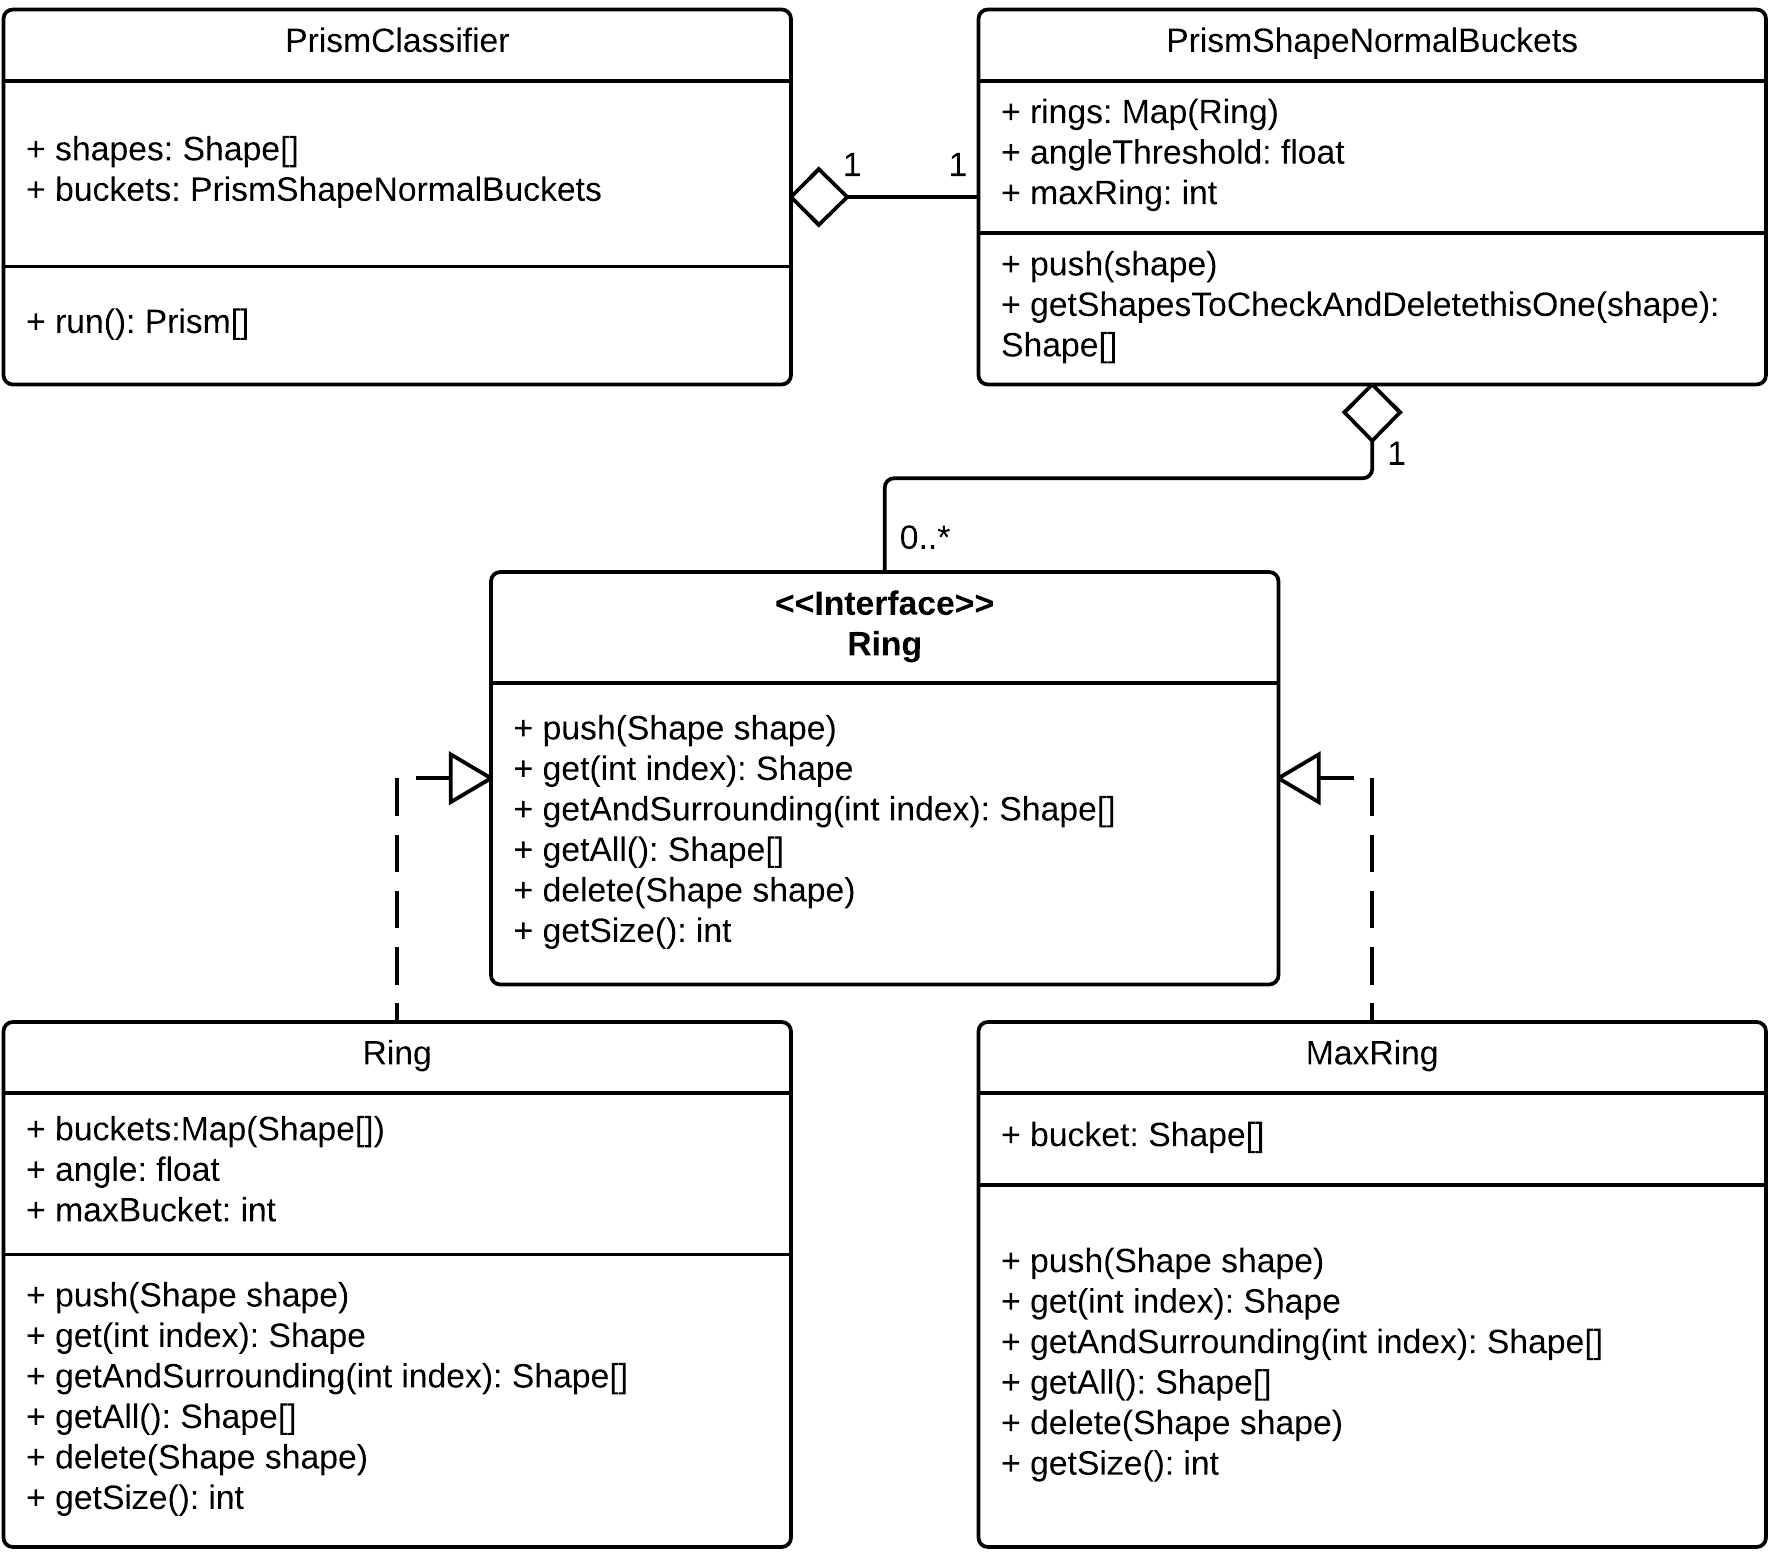
\includegraphics[width=1.0\columnwidth]{Images/04-prismClassifier.png}
\caption{Class diagram of the PrismClassifier}
\label{fig:prismClassifierDiagram}
\end{figure}

\paragraph{PrismClassifier}

\begin{listing}[!h]
\centering
\begin{minted}[
linenos, breaklines
]{coffeescript}
run: ->
    return new Promise( (resolve) =>
        buckets = new PrismShapeNormalsBuckets(_angleThreshold)

        @_putIntoBuckets @shapes, buckets

        prisms = @_detectPrisms @shapes, buckets

        log.debug("PrismClassifier found " + prisms.length + " prisms")

        resolve(prisms)
    )
\end{minted}
\caption{run method of the PrismClassifier}
\label{lst:PrismClassifierRun}
\end{listing}

Listing~\ref{lst:PrismClassifierRun} shows the implementation of the \emph{PrismClassifier} run method:

At first the normal buckets are initialised with an angle threshold as described in section \emph{Bucket System}. These values are stored in the global config with \emph{\_angleThreshold} $ = 0.15 = 8.6\degree $, previously labeled $\phi$, so shapes with an angle  of 8.6\textdegree \hspace{1pt} will be considered parallel.

Then all shapes are put into the corresponding buckets. This is done by iterating over all shapes and passing them to the bucket system which handles the classification on its own.

Next we iterate over all shapes again while requesting the potential parallel shapes from the bucket system. The shapes are checked with the given threshold and a \emph{prism} is created in case of parallelism.

At the end a set of all prisms is returned which can be used for further primitive classification.


\paragraph{Prism Shape Normals Buckets}

\emph{PrismShapeNormalsBuckets} is based on the specification in Section~\sectionref{sec:PrismBucketSystem} Bucket System: It divides a hemisphere into rings with buckets and is initialised with the angle threshold.

The constructor saves the angle threshold, instantiates the rings as a javascript map and calculates the maximum ring index $I_{MaxRing}$.

It provides two functions used by the classifier: \\
\emph{push} and \emph{getShapesToCheckAndDeleteThisOne}.

\emph{push} takes a \emph{Shape} and puts it in the corresponding ring. At first it transforms its normal into the hemisphere. Then the ring index $ I_{Ring} $ is calculated. If the ring is not initialised yet it gets created and \emph{ring.push(shape)} is called to sort the \emph{Shape} into the corresponding bucket.

\emph{getShapesToCheckAndDeleteThisOne} takes a \emph{Shape} and removes it from the bucket system because it will be checked for all possible prisms by the classifier and should not be returned as a potential parallel shape in another pass. Then it returns an array of all \emph{Shapes} lying in the same and the surrounding buckets: It requests the corresponding buckets from the ring with the shape's ring index $ I_{Ring} $ and the ring above and beneath.

While determining the surrounding rings following special cases need to be considered:

First: The ring with the maximum index $I_{MaxRing}$ is only adjacent to the ring underneath, because it is the highest ring on top of the hemisphere. It is not separated into different buckets and serves as a single bucket which is adjacent to all buckets in the ring underneath.

Second: The ring with index 0 "is adjacent to itself" because the unit sphere got transformed into a hemisphere. Therefore the buckets 180° around have to be taken into account for parallelism checks. Take two normals with the same x, y coordinates and a negated z value that span an angle smaller $ \phi $: $\vec{n_{1}} = (x, y, z)$ and $\vec{n_{2}} = (x, y, -z)$ with $z > 0$. Consequently $\vec{n_{1}}$ naturally lies in ring 0 and $\vec{n_{2}}$ gets negated to fit into the hemisphere. The negated normal is $\vec{n_{2}}' = (-x, -y, z) $ and lies also in ring 0 but in the opposite bucket 180° away.


\paragraph{Ring}

A \emph{Ring} contains buckets as a javascript map and is initialized with an index $ I_{Ring} $ and the angle threshold $ \phi$. With these the angle $ \gamma $ and the maximum bucket index $ I_{MaxBucket} $ are calculated as described in Section~\sectionref{sec:PrismBucketSystem}. It provides the methods \emph{push}, \emph{get}, \emph{getAndSurrounding}, \emph{getAll}, \emph{delete} and \emph{getSize}.

The method \emph{push} sorts a given shape into the corresponding bucket, \emph{get} returns all shapes of a bucket with a given index, \emph{getAndSurrounding} returns the same and additionaly the two neighboring buckets while \emph{getAll} returns all shapes that lie in that ring. With \emph{delete} a given \emph{Shape} is removed from the ring and \emph{getSize} returns the amount of \emph{Shapes} that lie in that ring.


\paragraph{MaxRing} The \emph{MaxRing} is only instanced once and is the ring with index $ I_{RingMax} $. It provides the same methods as a \emph{Ring} but with adapted behaviour.

\paragraph{Prism}

A \emph{Prism} contains two parallel shapes that span a prism. In future work this should be extended by the lateral surface which is not handled yet.

\subsubsection{Future Work}
\label{sec:PrismFutureWork}

\paragraph{Planes} \emph{Planes} from the \emph{PlaneClassifier} should be taken into account in addition to the shapes. Ideally the \emph{PlaneClassifier} detects noisy planes that are not represented as \emph{Shapes}. Therefore a better approximation of the original model could be achieved.

\paragraph{Lateral Surface} The lateral surface of the prism has yet to be identified and added to the prism structure. This is needed for further operations and more specific classifications of the prism. For example for classifying a cube the surrounding sides have to be known.

\paragraph{Scoring} Prism scoring is not implemented yet. To rate a prism the actual angle between the two nearly parallel shapes have to be considered. If scoring is implemented the angle threshold for parallelism can be adjusted to a much higher value while big variations to 0° will be reflected in the score.





















\subsection{Other Primitives}
In addition to the just mentioned objects any other primitive can be included in the search with RANSAC. \\
For this a number of minimum support points is needed. This number of points needs to suffice to reconstruct the object. \\
Other points from the dataset can then be tested if they support the constructed object. 
\section{Problems with Non-Point-Cloud Input}
In our use case we do not get a point-cloud as input. Instead we operate on the much fewer points in a polygon mesh.\\
This has large influence on the threshold values that are used. The values taken from CGAL almost never achieve the desired results. We tried to find new values for any model which turned out to be infeasible. Therefore we tried adjusting the thresholds based on the number of vertices in the mesh or the volume of the bounding box. We have not encountered a working combination yet. This is a problem that needs to be tackled in future work.
\end{document}